%
%Не забыть:
%--------------------------------------
%Вставить колонтитулы, поменять название на титульнике



%--------------------------------------

\documentclass[a4paper, 12pt]{article} 

%--------------------------------------
%Russian-specific packages
%--------------------------------------
%\usepackage[warn]{mathtext}
\usepackage[T2A]{fontenc}
\usepackage[utf8]{inputenc}
\usepackage[english,russian]{babel}
\usepackage[intlimits]{amsmath}
\usepackage{esint}
%--------------------------------------
%Hyphenation rules
%--------------------------------------
\usepackage{hyphenat}
\hyphenation{ма-те-ма-ти-ка вос-ста-нав-ли-вать}
%--------------------------------------
%Packages
%--------------------------------------
\usepackage{amsmath}
\usepackage{amssymb}
\usepackage{amsfonts}
\usepackage{amsthm}
\usepackage{latexsym}
\usepackage{mathtools}
\usepackage{etoolbox}%Булевые операторы
\usepackage{extsizes}%Выставление произвольного шрифта в \documentclass
\usepackage{geometry}%Разметка листа
\usepackage{indentfirst}
\usepackage{wrapfig}%Создание обтекаемых текстом объектов
\usepackage{fancyhdr}%Создание колонтитулов
\usepackage{setspace}%Настройка интерлиньяжа
\usepackage{lastpage}%Вывод номера последней страницы в документе, \lastpage
\usepackage{soul}%Изменение параметров начертания
\usepackage{hyperref}%Две строчки с настройкой гиперссылок внутри получаеммого
\usepackage[usenames,dvipsnames,svgnames,table,rgb]{xcolor}% pdf-документа
\usepackage{multicol}%Позволяет писать текст в несколько колонок
\usepackage{cite}%Работа с библиографией
\usepackage{subfigure}% Человеческая вставка нескольких картинок
\usepackage{tikz}%Рисование рисунков
\usepackage{float}% Возможность ставить H в положениях картинки
% Для картинок Моти
\usepackage{misccorr}
\usepackage{lscape}
\usepackage{cmap}



\usepackage{graphicx,xcolor}
\graphicspath{{Pictures/}}
\DeclareGraphicsExtensions{.pdf,.png,.jpg}

%----------------------------------------
%Список окружений
%----------------------------------------
\newenvironment {theor}[2]
{\smallskip \par \textbf{#1.} \textit{#2}  \par $\blacktriangleleft$}
{\flushright{$\blacktriangleright$} \medskip \par} %лемма/теорема с доказательством
\newenvironment {proofn}
{\par $\blacktriangleleft$}
{$\blacktriangleright$ \par} %доказательство
%----------------------------------------
%Список команд
%----------------------------------------
\newcommand{\grad}
{\mathop{\mathrm{grad}}\nolimits\,} %градиент

\newcommand{\diver}
{\mathop{\mathrm{div}}\nolimits\,} %дивергенция

\newcommand{\rot}
{\ensuremath{\mathrm{rot}}\,}

\newcommand{\Def}[1]
{\underline{\textbf{#1}}} %определение

\newcommand{\RN}[1]
{\MakeUppercase{\romannumeral #1}} %римские цифры

\newcommand {\theornp}[2]
{\textbf{#1.} \textit{ #2} \par} %Написание леммы/теоремы без доказательства

\newcommand{\qrq}
{\ensuremath{\quad \Rightarrow \quad}} %Человеческий знак следствия

\newcommand{\qlrq}
{\ensuremath{\quad \Leftrightarrow \quad}} %Человеческий знак равносильности

\renewcommand{\phi}{\varphi} %Нормальный знак фи

\newcommand{\me}
{\ensuremath{\mathbb{E}}}

\newcommand{\md}
{\ensuremath{\mathbb{D}}}



%\renewcommand{\vec}{\overline}




%----------------------------------------
%Разметка листа
%----------------------------------------
\geometry{top = 3cm}
\geometry{bottom = 2cm}
\geometry{left = 1.5cm}
\geometry{right = 1.5cm}
%----------------------------------------
%Колонтитулы
%----------------------------------------
\pagestyle{fancy}%Создание колонтитулов
\fancyhead{}
%\fancyfoot{}
%----------------------------------------
%Интерлиньяж (расстояния между строчками)
%----------------------------------------
%\onehalfspacing -- интерлиньяж 1.5
%\doublespacing -- интерлиньяж 2
%----------------------------------------
%Настройка гиперссылок
%----------------------------------------
\hypersetup{				% Гиперссылки
	unicode=true,           % русские буквы в раздела PDF
	pdftitle={Заголовок},   % Заголовок
	pdfauthor={Автор},      % Автор
	pdfsubject={Тема},      % Тема
	pdfcreator={Создатель}, % Создатель
	pdfproducer={Производитель}, % Производитель
	pdfkeywords={keyword1} {key2} {key3}, % Ключевые слова
	colorlinks=true,       	% false: ссылки в рамках; true: цветные ссылки
	linkcolor=blue,          % внутренние ссылки
	citecolor=blue,        % на библиографию
	filecolor=magenta,      % на файлы
	urlcolor=cyan           % на URL
}
%----------------------------------------
%Работа с библиографией (как бич)
%----------------------------------------
\renewcommand{\refname}{Список литературы}%Изменение названия списка литературы для article
%\renewcommand{\bibname}{Список литературы}%Изменение названия списка литературы для book и report
%----------------------------------------
\begin{document}
	\begin{titlepage}
		\begin{center}
			$$$$
			$$$$
			$$$$
			$$$$
			{\Large{НАЦИОНАЛЬНЫЙ ИССЛЕДОВАТЕЛЬСКИЙ УНИВЕРСИТЕТ}}\\
			\vspace{0.1cm}
			{\Large{ВЫСШАЯ ШКОЛА ЭКОНОМИКИ}}\\
			\vspace{0.25cm}
			{\large{Факультет физики}}\\
			\vspace{5.5cm}
			{\Huge\textbf{{Лабораторные работы по спектроскопии и дифракции}}}\\%Общее название
			\vspace{1cm}
			{Работу выполнил студент 3 курса}\\
			{Захаров Сергей Дмитриевич}
			\vfill
			
\includegraphics[width = 0.2\textwidth]{HSElogo}\\
			\vfill
			Москва\\
			2021
		\end{center}
	\end{titlepage}
	
\tableofcontents

\newpage

\section{Постановка цели}

\subsection{Оже-спектроскопия}

В качестве исследуемого вещества нам был предложен неизвестный сыпучий образец, спрессованный в форму ломкой цилиндрической таблетки. Предлагалось подготовить ее для внесения в вакуумную камеру, после чего внести в нее и получить Оже-спектр, после чего путем его анализа постараться определить, из каких элементов образец состоит.

\subsection{Сканирующая туннельная микроскопия}

Было решено на уже внесенном в вакуум графите получить обзорный кадр и определить высоту ступеньки. Забегая вперед, в ходе эксперимента проявился т.н. муаровый узор, возникающий при наложении двух периодических сетчатых рисунков, например, слоев решетки графита, поэтому было также предложено по нему определить взаимное расположение слоев, дающих рисунок.

\subsection{Сканирующая туннельная спектроскопия}

Также на уже внесенном в вакуум графите было предложено получить вольт-амперную характеристику (ВАХ) туннельного тока от напряжения.

\section{Оже-спектроскопия}

\subsection{Описание эффекта}

Мы пользуемся тем фактом, что энергия связи электронов глубоких оболочек атома чувствительна к природе элемента, что позволяет, измеряя кинетическую энергию эмитированных с поверхности под действием фотонной или электронной бомбардировки, получать информацию об \textbf{элементном} составе поверхности. Мы также пользуемся тем, что электроны с кинетической энергией 15-1000~эВ обладают очень маленькими длинами свободного пробега в веществе, что позволяет получать информацию о поверхности.

Мы рассматриваем оже-пики, которые появляются вследствие т.н. Оже-процесса. Схема процесса представлена на рисунке \ref{fig:1_diag} и состоит из трех этапов. Сперва первичный электрон с энергией порядка 2-3~кЭв выбивает электрон с оболочки атома, образуя тем самым вакансию (а). После этого происходит релаксация за счет внутреннего перехода электрона с более высокого уровня на получившуюся вакансию (б). Наконец, испускается Оже-электрон, который мы детектируем и кинетическую энергию которого мы измеряем (в).

\begin{figure}[H]
	\centering
	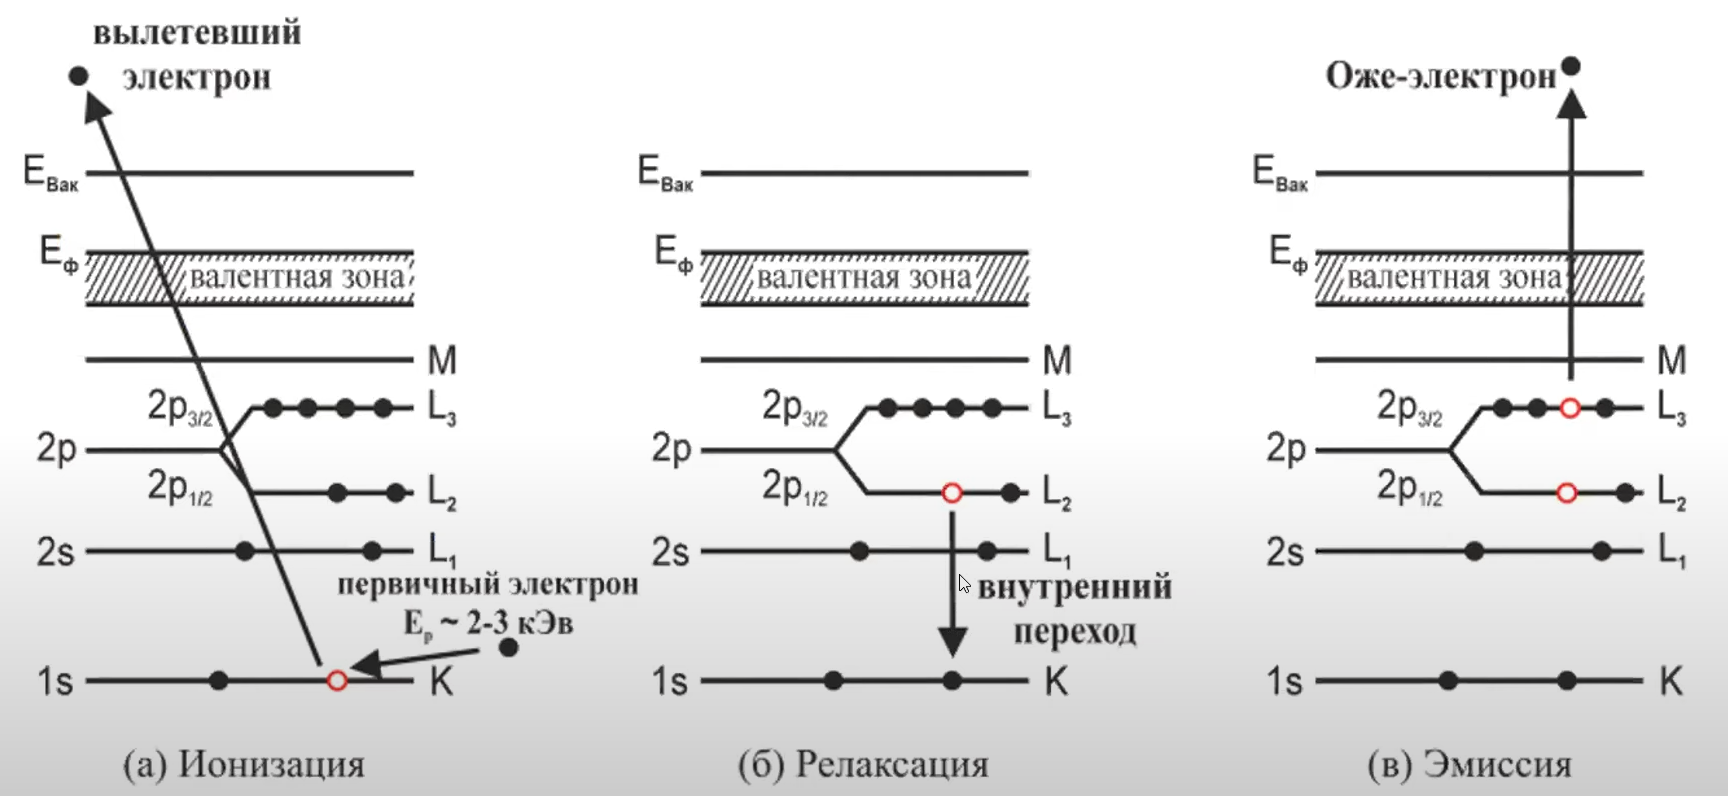
\includegraphics[width=0.7\linewidth]{1_diag}
	\caption{Схематическая иллюстрация оже-процесса из \cite{Auge_diag}.}
	\label{fig:1_diag}
\end{figure}

\subsection{Подготовка образца}

Первоначально предлагалось закрепить образец на держателе с помощью танталовой нити с использованием контактной сварки, однако спустя несколько попыток было решено, что данный способ при отсутствии должной практики крайне сложен в практическом исполнении, принимая во внимание тот факт, что образец был цилиндрической формы. По этой причине было решено <<накрыть>> образец танталовой пластиной, предварительно просверлив в ней отверстие достаточного диаметра для получения Оже-спектра и сделав <<ножки>>, с помощью которых образец бы держался между пластинами (см. рисунок). % ссылка на рисунок

%\begin{figure}[H]
%	\centering
%	\includegraphics[width=0.7\linewidth]{1_fastening}
%	\caption{Крепление образца с помощью танталовой пластины.}
%	\label{fig:1_fastening}
%\end{figure}

\subsection{Анализ Оже-спектра}

Изначально был получен Оже-спектр при бомбардировке образца электронами с энергией 3000~эВ с помощью установки, описанной в \cite{Auger_spectr}. С учетом возможности наличия т.н. пиков потерь, которые находятся в той же области, что и оже-пики, было решено проверить их присутствие с помощью увеличения энергии бомбардирующих электронов на 500~эВ. В таком случае Оже-пики, которые являются характеристикой вещества, должны были бы остаться на месте, а пики потерь --- сместиться. Из рисунка \ref{fig:1_Auge_double} видно, что смещения ни одного из пиков не наблюдается, что свидетельствует о том, что все пики являются оже-пиками.

В силу совпадения оже-спектров анализ проводился только спектра 3000~эВ. Однако в более <<далекой>> по энергиям части спектра для того, чтобы лучше разрешить пики, оказался полезен и спектр 3500~эВ. Понятно, что в идеале хотелось бы иметь спектр 5000~эВ, пики с которого соответствовали бы, как и пики с 3000~эВ, каталожным, однако это оказалось невозможно по независящим от нас техническим причинам. Проанализированный спектр 3000~эВ представлен на рисунке \ref{fig:1_Auge_3000}.

Как было сказано, спектр 3500~эВ оказался полезен в <<дальней>> части спектра: с его помощью был уточнен пик, предположительно, тулия. Кроме того, благодаря тому, что это сканирование мы запустили с меньшего нижнего порога по энергиям, из него также можно было вытащить один дополнительный пик в начале, который оказался натриевым. Эти два ненайденных с помощью спектра 3000~эВ пика указаны на спектре 3500~эВ на рисунке \ref{fig:1_Auge_3500}. 

В качестве каталожных спектров были взяты спектры из \cite{Auger}.

\section{Сканирующая туннельная микроскопия}

Для сканирования, как было сказано выше, был выбран графитовый образец. Сканирование проводилось на установке GPI-300 \cite{STM}.

\subsection{Измерение высоты ступеньки и получение обзорного СТМ-кадра}

С помощью последовательного сканирования различных областей, была найдена область с несколькими ступенями. На основании полученных данных возможно измерить высоту ступени, которая оказалась равной $4.5$ \AA. Полученное изображение представлено на рисунке \ref{fig:2_step}. График перепада высот на исследованной ступеньке указан на рисунке \ref{fig:2_step_anal}.

\subsection{Получение атомной структуры}

Были получены кадры с различным увеличением атомной структуры, которые представлены на рисунках \ref{fig:2_small_atoms} и \ref{fig:2_big_atoms}.

\subsection{Зависимость СТМ-изображения атомной структуры от напряжения}

На одном и том же участке было проведено несколько последовательных сканирований при различных напряжениях с целью найти какую-то зависимость качества изображения от этого напряжения. В результате было определено, что явной зависимости нет, а параметры необходимо подбирать индивидуально. Полученные кадры представлены на рисунке \ref{fig:2_different_volt}, а также на рисунке \ref{fig:2_big_atoms}.

\subsection{Наблюдение муара}

Увиденный нами муар при различных увеличениях представлен на рисунке \ref{fig:2_muar}. Проанализировать его и получить, каким конкретно поворотом плоскостей он вызван, однако, не удалось.

\section{Сканирующая туннельная спектроскопия}

На уже использованном для СТМ графитовом образце было снято несколько ВАХ на одном и том же месте. После анализа результатов была выбрана наименее зашумленная серия, которая после этого была дополнительно отфильтрована. Полученная ВАХ (исходная и после фильтра) представлена на рисунке \ref{fig:3_STS}. Видно, что на ней все еще достаточно много шумов. Чтобы это улучшить, вероятно, стоит изначально подводить иглу ближе к образу (т.е. менять $U_{\text{base}}$), а также уменьшить шаг по напряжению.

\section{Выводы}

В результате проведения лабораторной работы:

\begin{enumerate}
	\item Был расшифрован Оже-спектр неизвестного образца. Предположительно он состоит из натрия, фтора, тулия и иттрия. Пики углерода и кислорода принимается, что происходят из остатков газа в вакуумной камере.
	
	\item Была измерена высота ступеньки на графитовом образце. Ее высота оказалась равной 4.5~\AA.
	
	\item Были получены различные СТМ-кадры, в том числе и обзорные, и кадры, отображающие атомную структуру.
	
	\item Был проведен эксперимент по поиску зависимости качества СТМ-изображения атомной структуры от напряжения, в ходе которого было установлено, что явной зависимости (например, чем больше напряжение, тем лучше качество изображения) не было выявлено.
	
	\item При сканировании был обнаружен муар, который, по всей видимости, вызывается поворотом двух (или более) слоев решетки относительно друг друга, однако смоделировать и проверить данную теорию возможным не представилось и остается одной из возможных задач будущей работы.
	
	\item Была получена ВАХ, которая отдаленно напоминает ВАХ, например, из \cite{Article}, однако она сильно зашумлена. В качестве вариантов решения проблемы в будущем были предложены более близкое подведение иглы к образцу и уменьшение шага по напряжению.
\end{enumerate}

\newpage

\begin{thebibliography}{2}
	
	\bibitem{Auger} Handbook of Auger Electron Spectroscopy. /  Lawrence E. Davis, Noel C. MacDonald, Paul W. Palmberg, Greald E. Riach, Roland E. Wever --- Physical Electrinics Industries, Inc., February 1976.
	
	\bibitem{Auger_spectr} Описание работы оже-спектрометра. / ??
	
	\bibitem{STM} Общее описание СТМ GPI-300. / ??
	
	\bibitem{Article} Scanning tunneling microscopy and spectroscopy of the electronic local density of states of graphite surfaces near monoatomic step edges. / Y. Niimi, T. Matsui, H. Kambara, K. Tagami, M. Tsukada, and Hiroshi Fukuyama --- Tokyo, Japan : Department of Physics, University of Tokyo, February 24, 2006.
	
	\bibitem{Auge_diag} Анализ поверхности методами Оже- и рентгеновской фотоэлектронной спектроскопии. / Бриггса Д., Сиха М.М.
	
\end{thebibliography}


\newpage

% Оже-спектры выношу отдельно, по одному на страницу, чтобы не сидеть "а че там написано"

\begin{figure}[H]
	\centering
	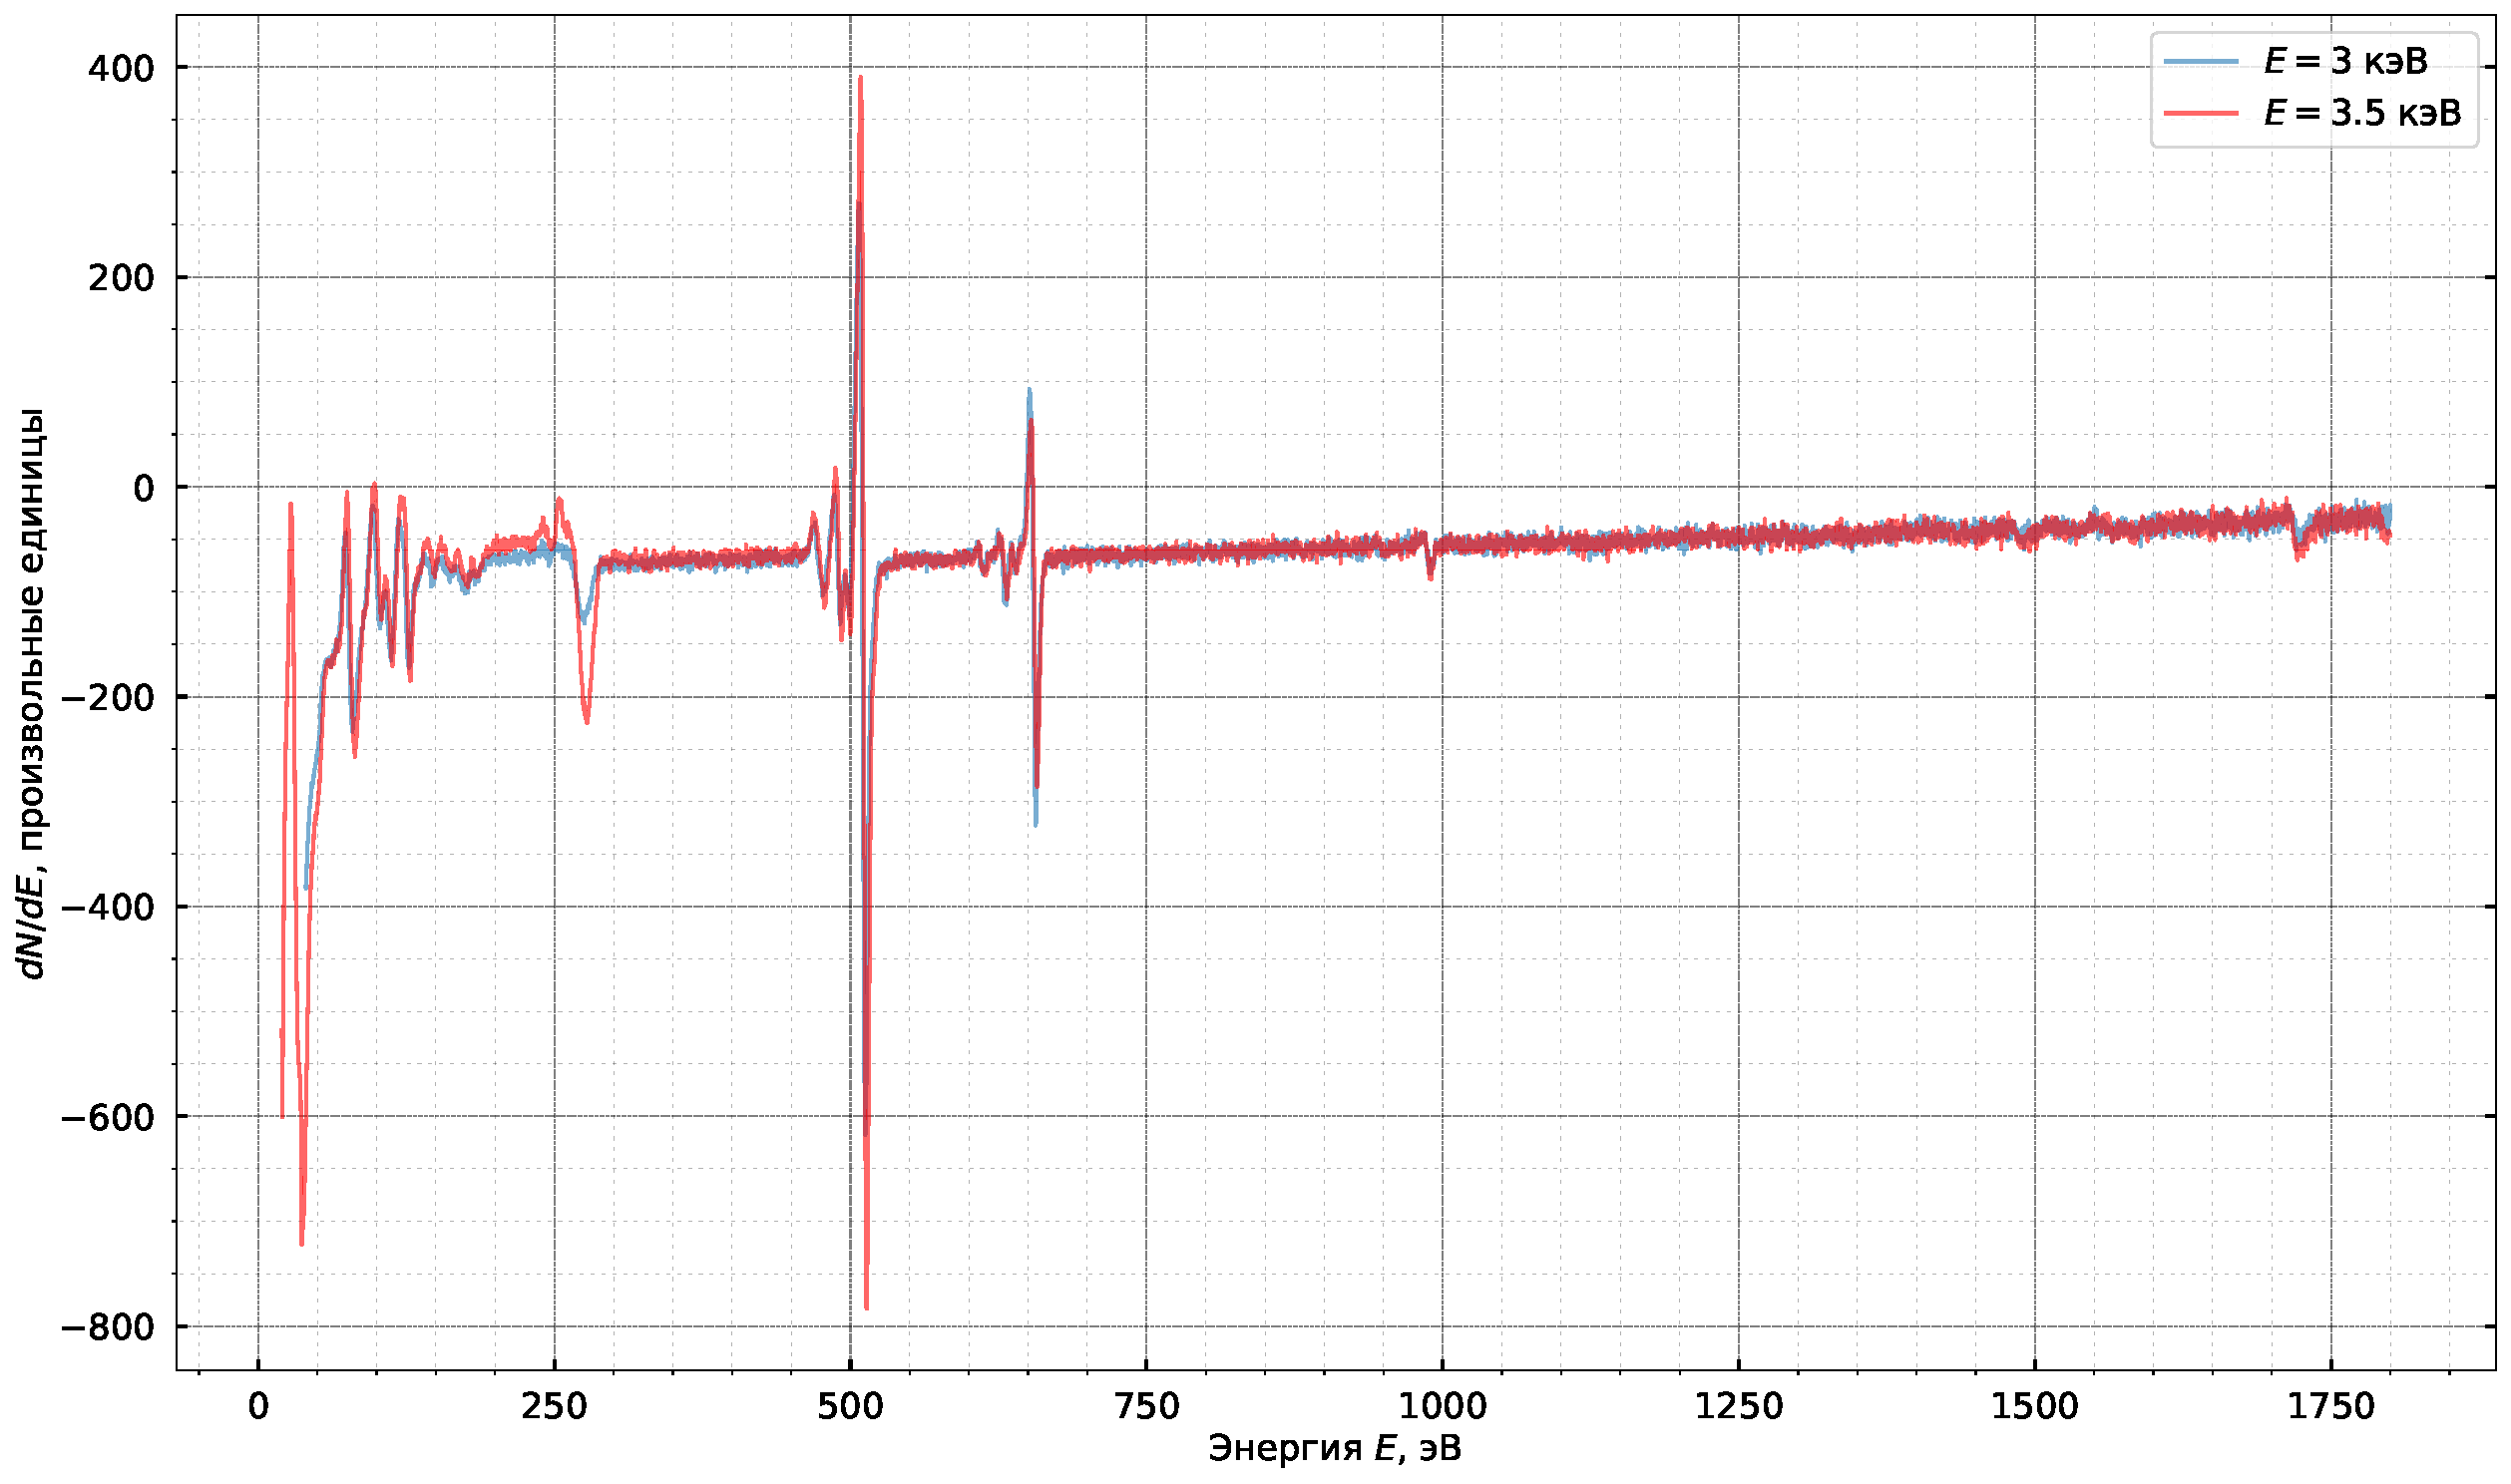
\includegraphics[width=1.3\linewidth, angle=-90]{1_Auge_double}
	\caption{Сравнение Оже-спектров, полученных при 3000~эВ и 3500~эВ.}
	\label{fig:1_Auge_double}
\end{figure}

\newpage

\begin{figure}[H]
	\centering
	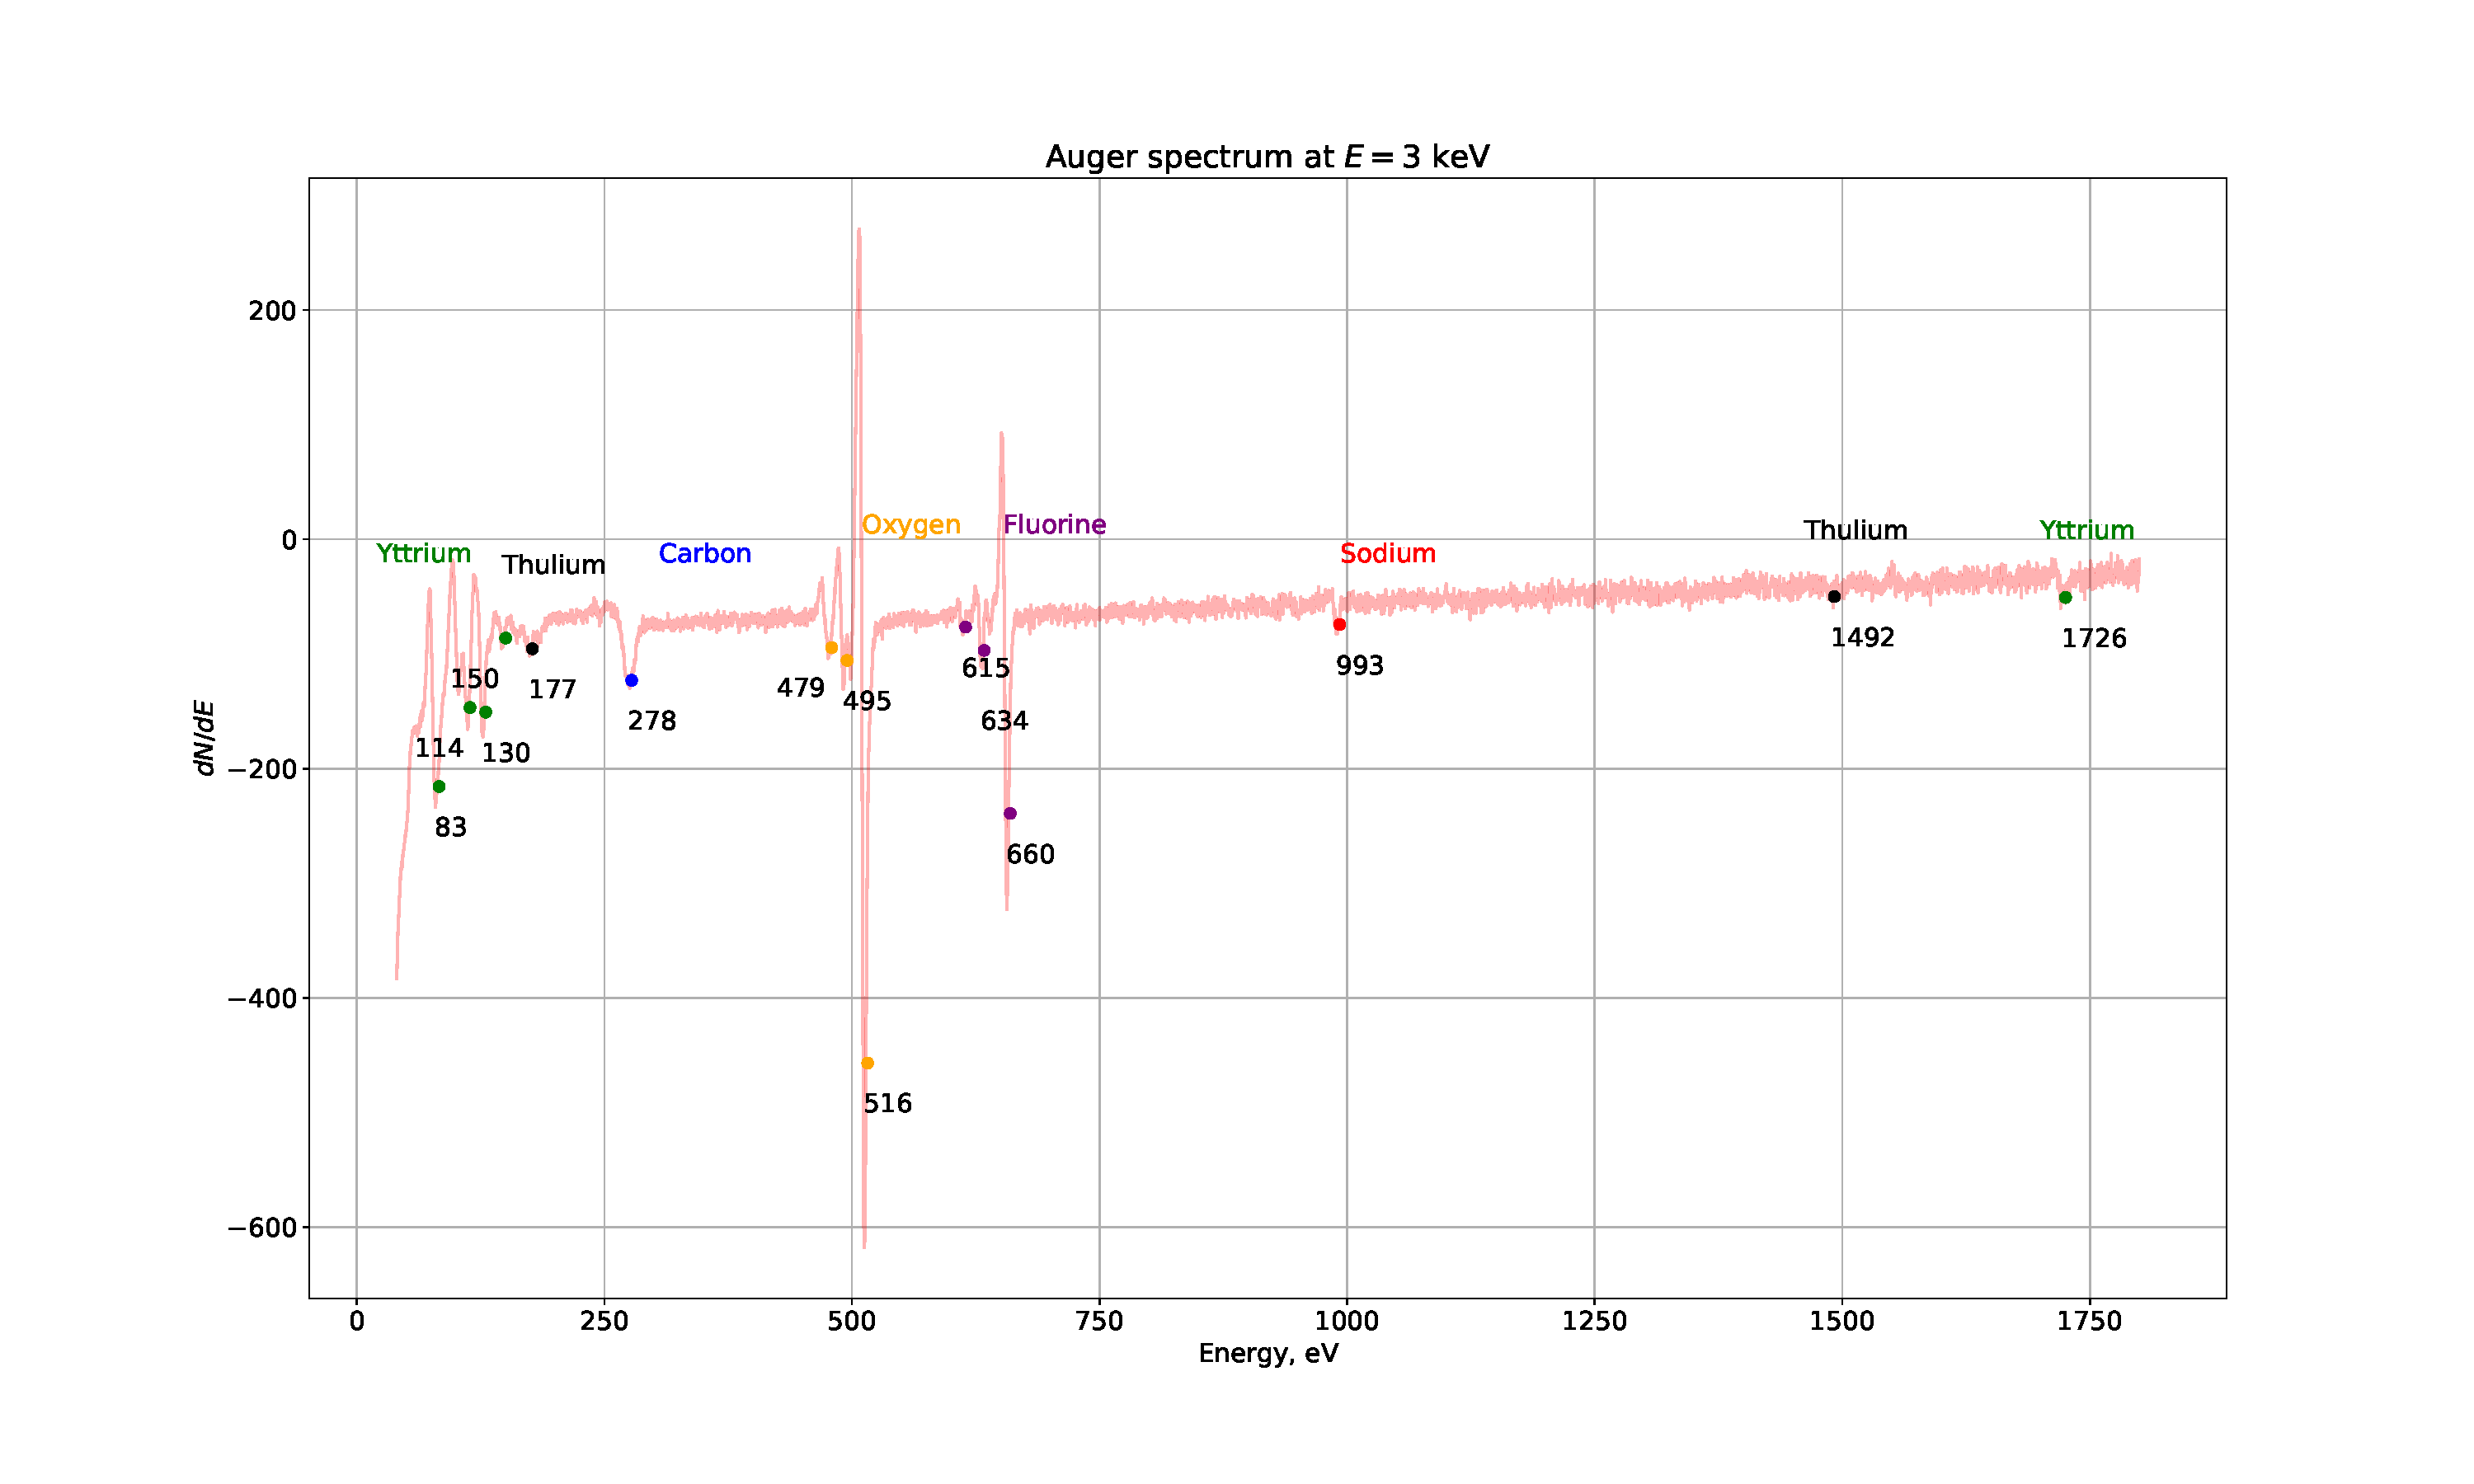
\includegraphics[width=1.3\linewidth, angle=-90]{1_Auge_3000}11
	\caption{Полученный Оже-спектр 3000~эВ с нанесенными названиями элементов, дающих пики.}
	\label{fig:1_Auge_3000}
\end{figure}

\newpage

\begin{figure}[H]
	\centering
	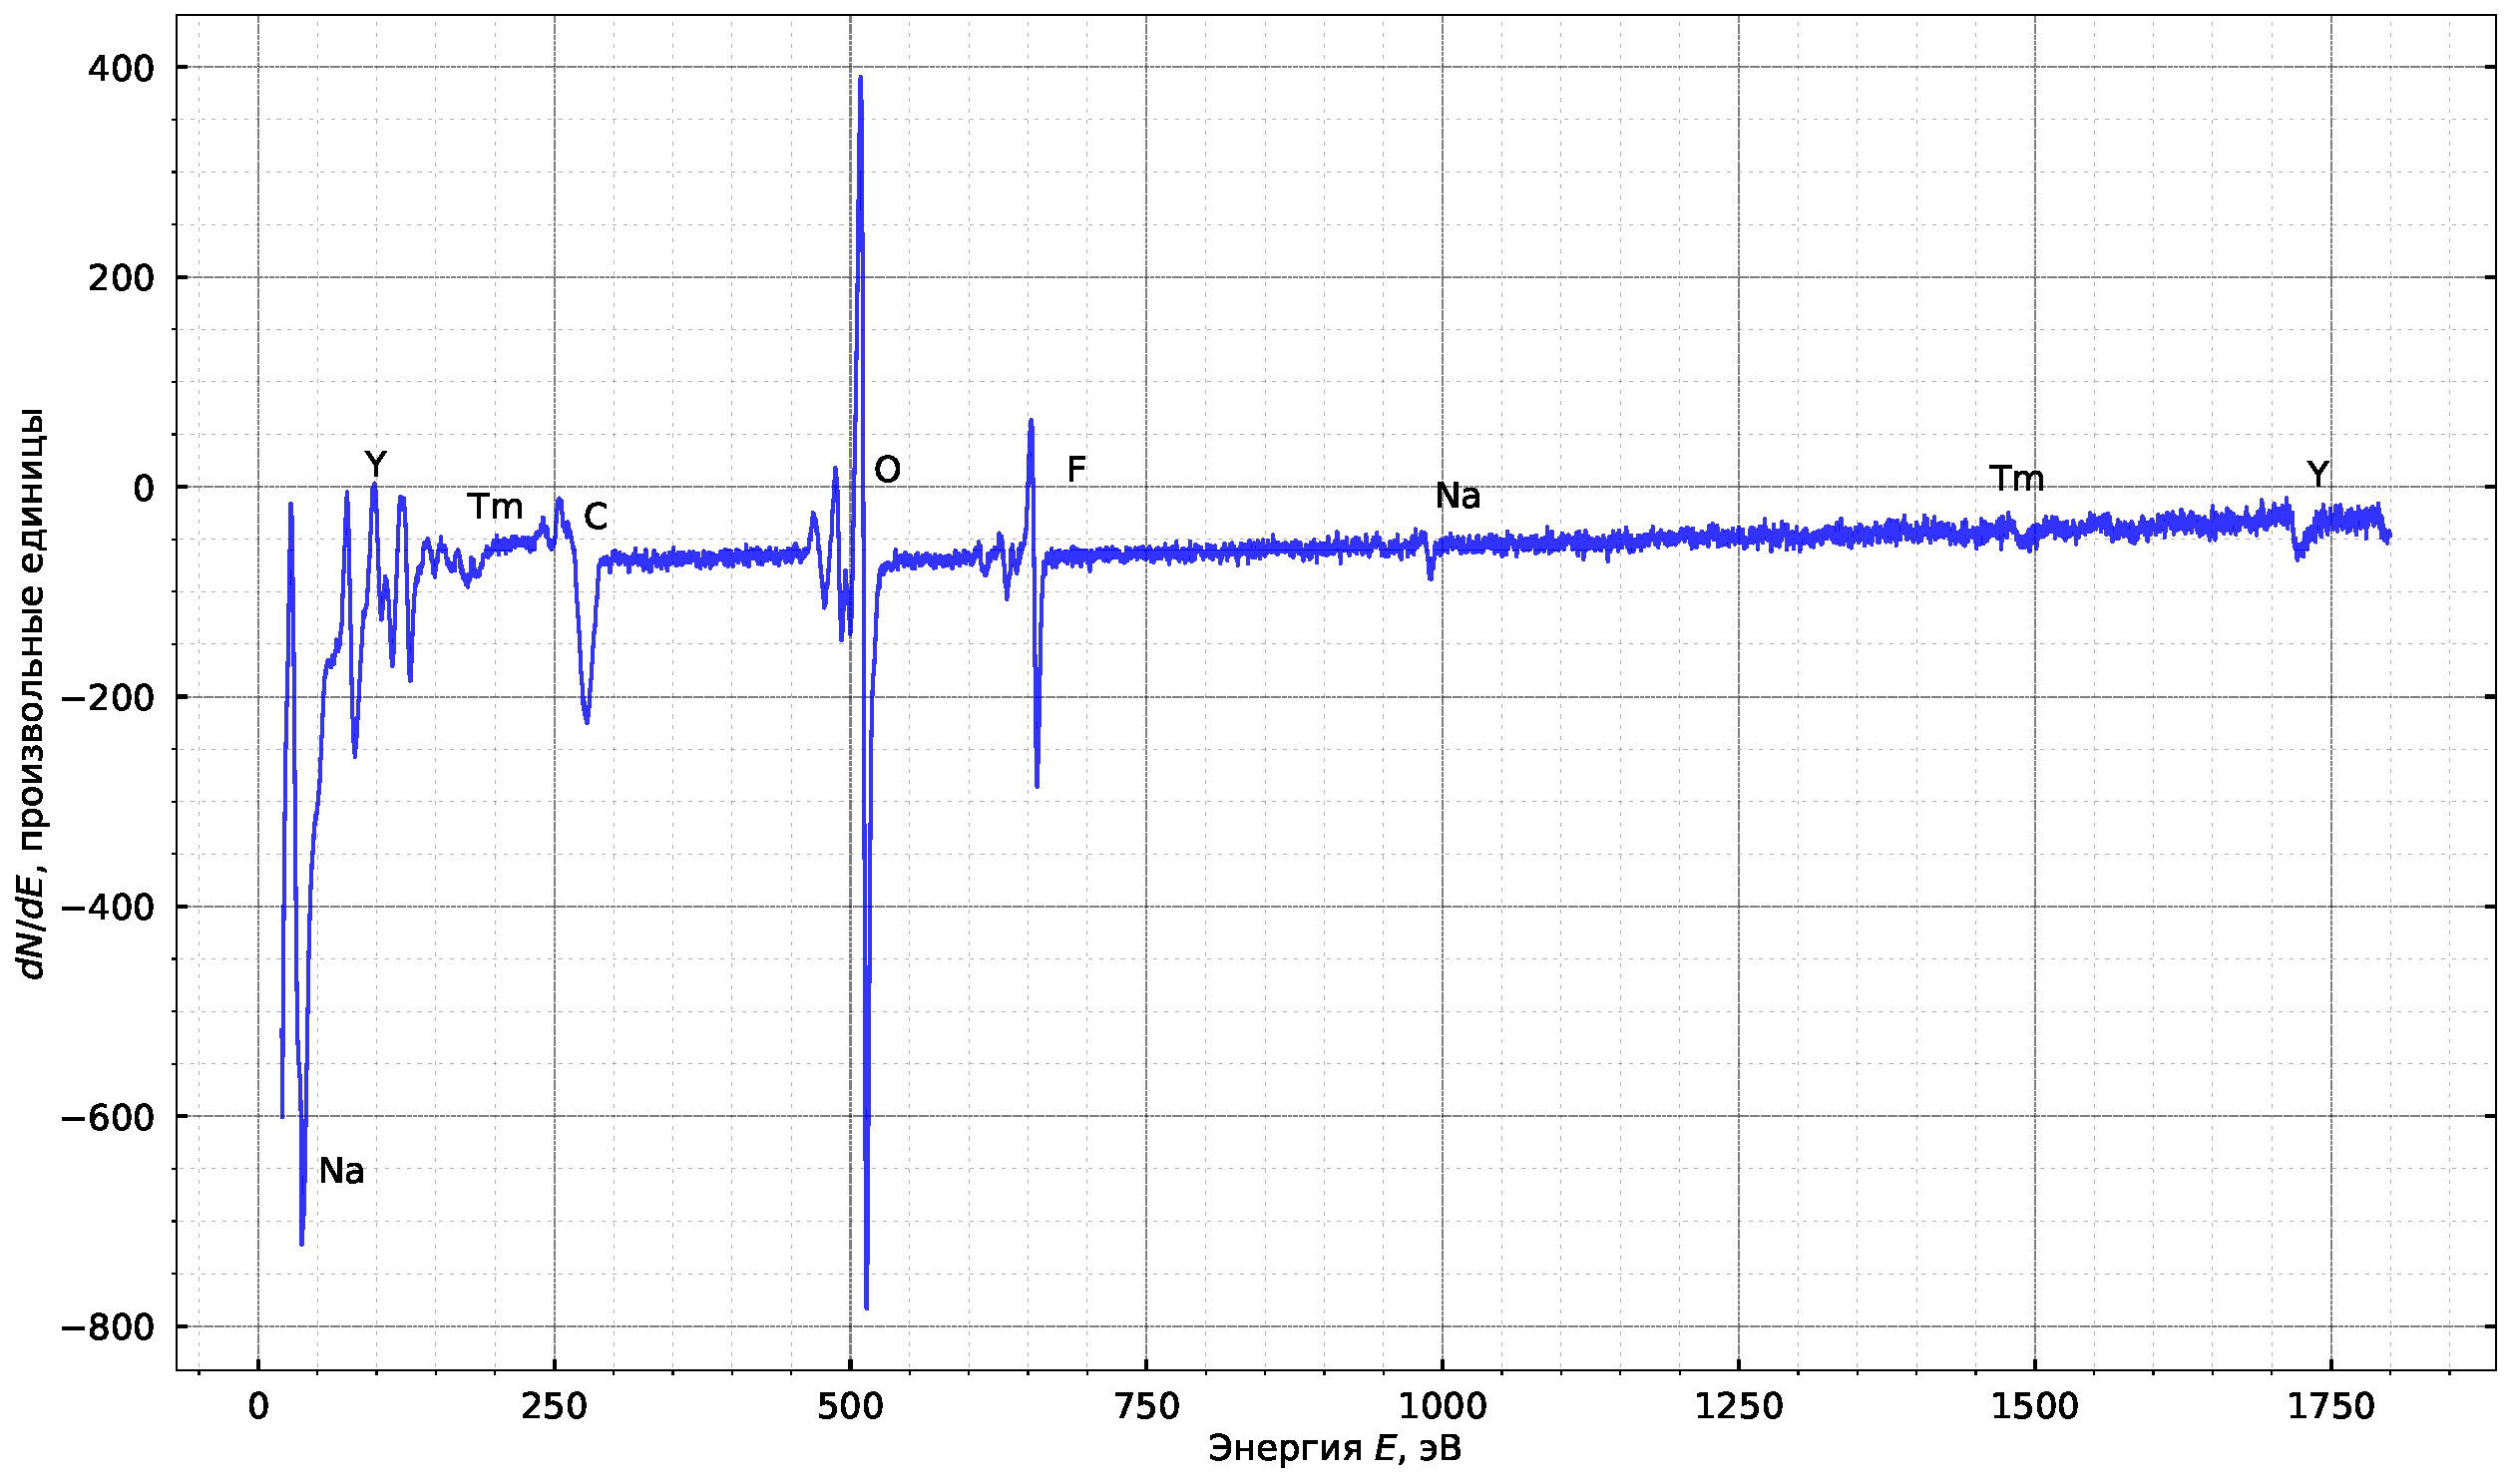
\includegraphics[width=1.3\linewidth, angle=-90]{1_Auge_3500}
	\caption{Полученный Оже-спектр 3000~эВ с нанесенными названиями элементов, дающих не найденные на 3000~эВ пики.}
	\label{fig:1_Auge_3500}
\end{figure}

\newpage

\begin{figure}[H]
	\centering
	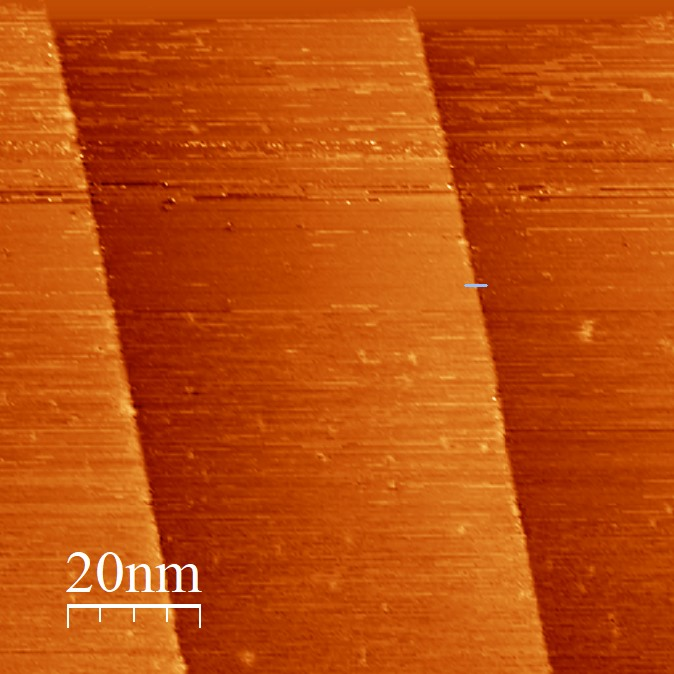
\includegraphics[width=0.6\linewidth]{2_step}
	\caption{СТМ-изображение ступенек на поверхности графита.}
	\label{fig:2_step}
\end{figure}

\begin{figure}[H]
	\centering
	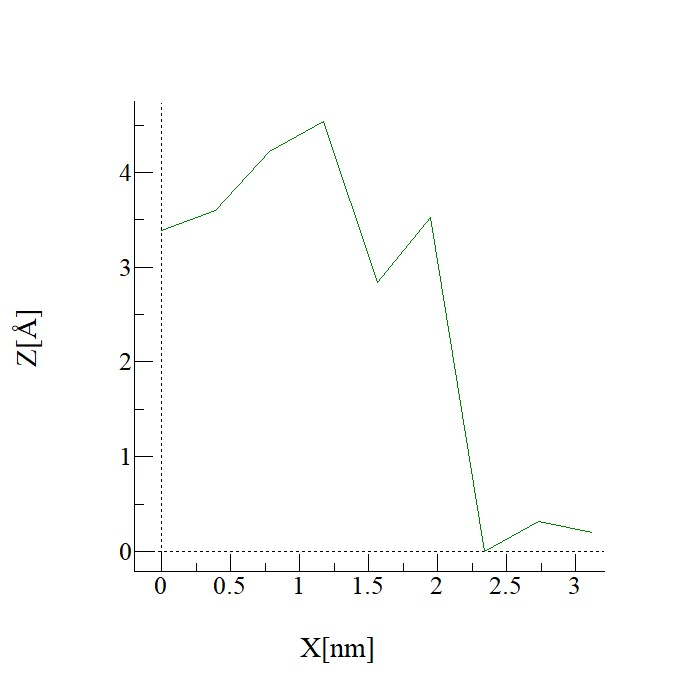
\includegraphics[width=0.6\linewidth]{2_step_anal}
	\caption{Перепад высот на ступени на поверхности графита.}
	\label{fig:2_step_anal}
\end{figure}

\begin{figure}[H]
	\centering
	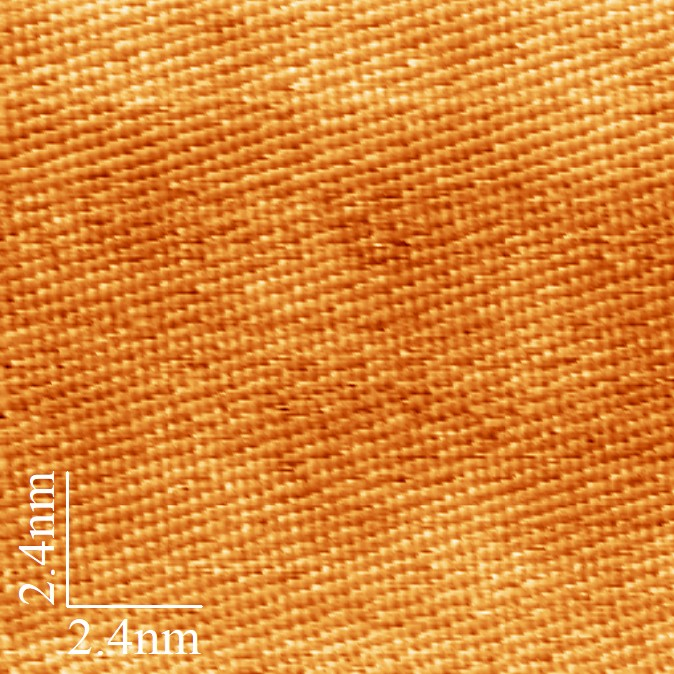
\includegraphics[width=0.6\linewidth]{2_small_atoms}
	\caption{СТМ-изображение атомной структуры.}
	\label{fig:2_small_atoms}
\end{figure}

\begin{figure}[H]
	\centering
	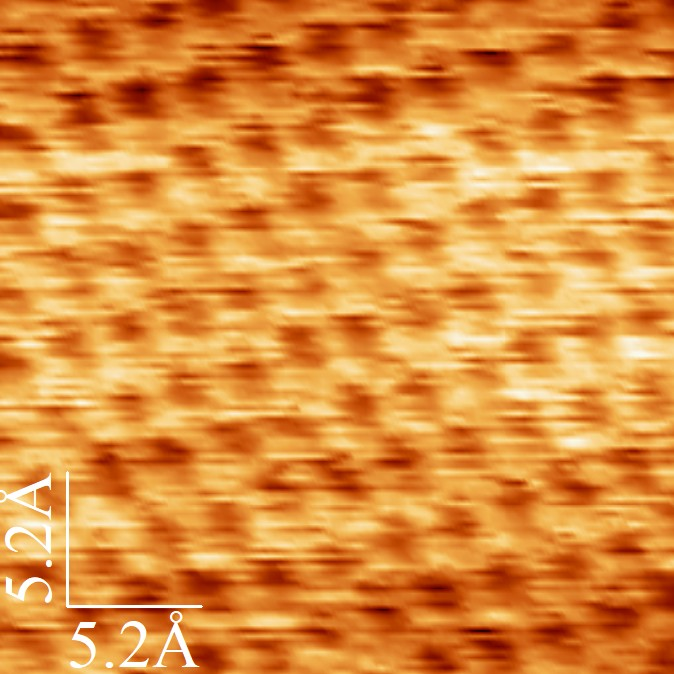
\includegraphics[width=0.6\linewidth]{2_big_atoms}
	\caption{СТМ-изображение атомной структуры (вблизи) при напряжении 199.863~мВ.}
	\label{fig:2_big_atoms}
\end{figure}

\begin{figure}[H]
	\centering
	\subfigure[]{
		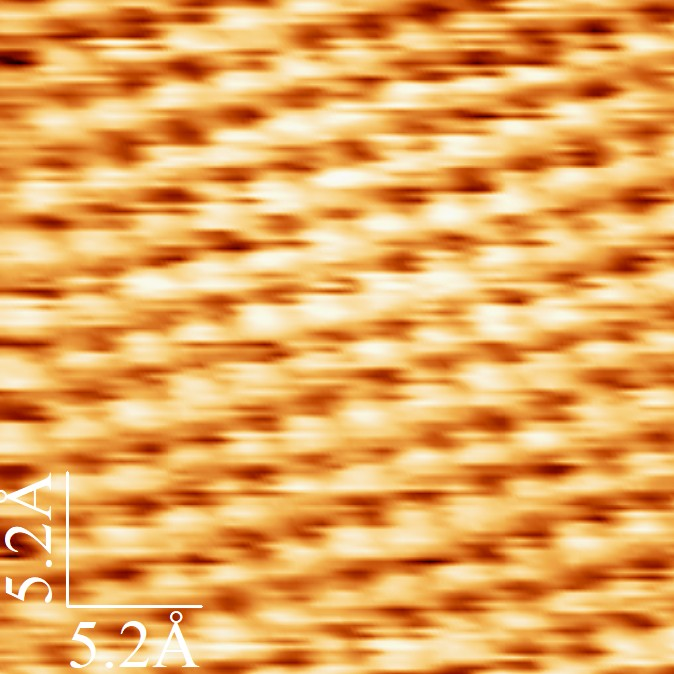
\includegraphics[width=0.4\linewidth]{2_25564}
	}	
	\subfigure[]{
		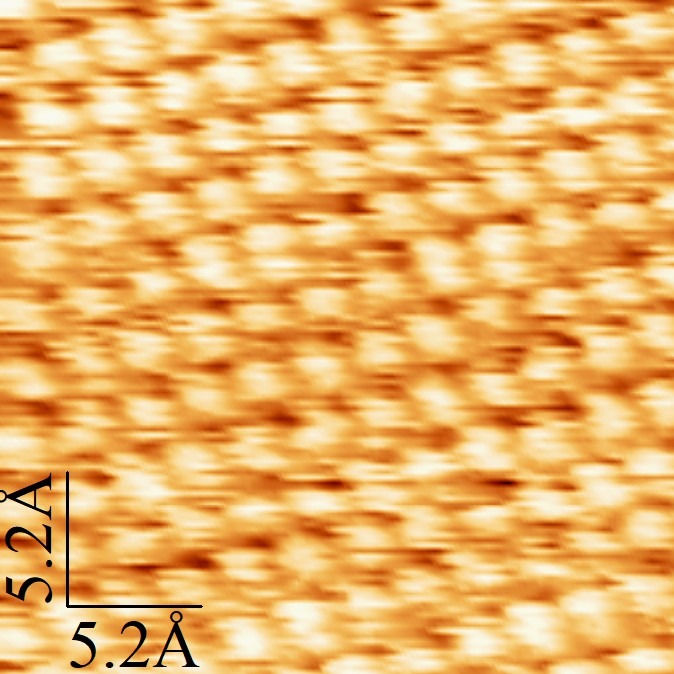
\includegraphics[width=0.4 \linewidth]{2_64408}
	}
	\subfigure[]{
		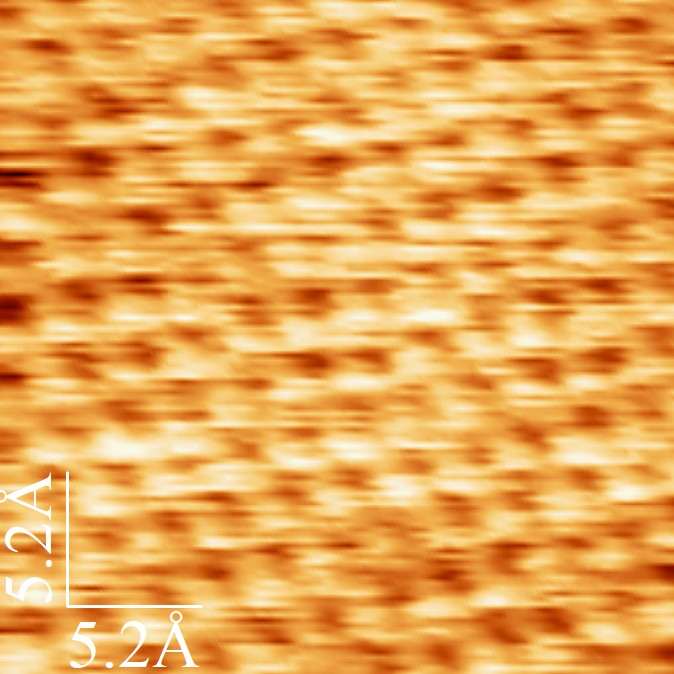
\includegraphics[width=0.4\linewidth]{2_93292}
	}	
	\subfigure[]{
		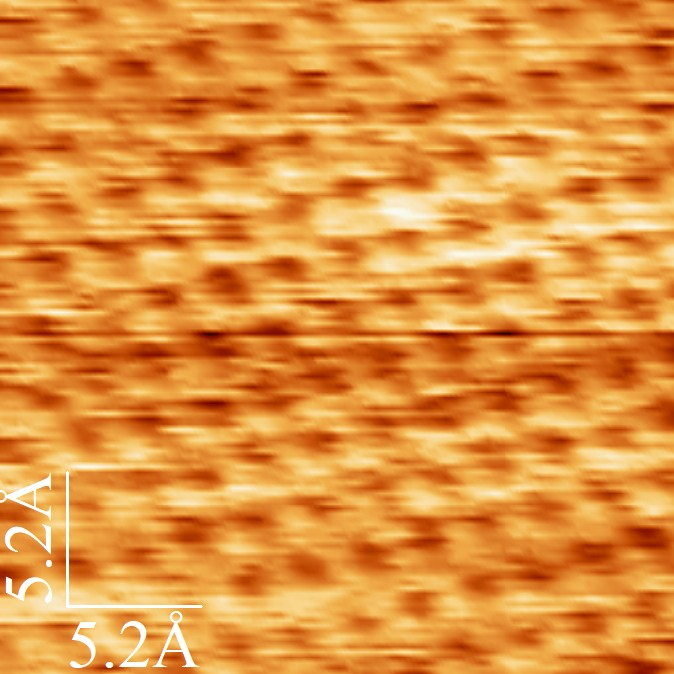
\includegraphics[width=0.4 \linewidth]{2_150064}
	}
	
	\caption{СТМ-изображение атомной структуры (вблизи) при различных напряжениях. Слева направо и сверху вниз при напряжении, соответственно: 25.6~мВ, 64.4~мВ, 93.3~мВ, 150.1~мВ.}
	\label{fig:2_different_volt}
\end{figure}

\begin{figure}[H]
	\centering
	\subfigure[]{
		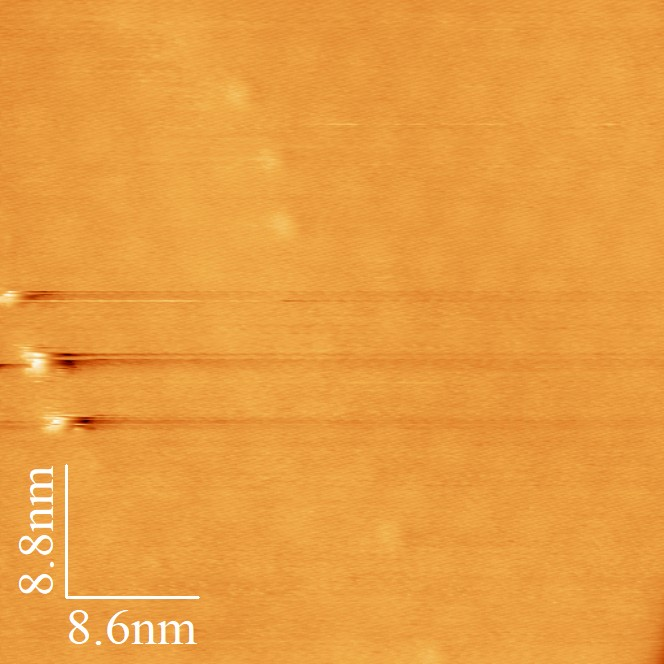
\includegraphics[width=0.45\linewidth]{2_muar}
	}
	\subfigure[]{
		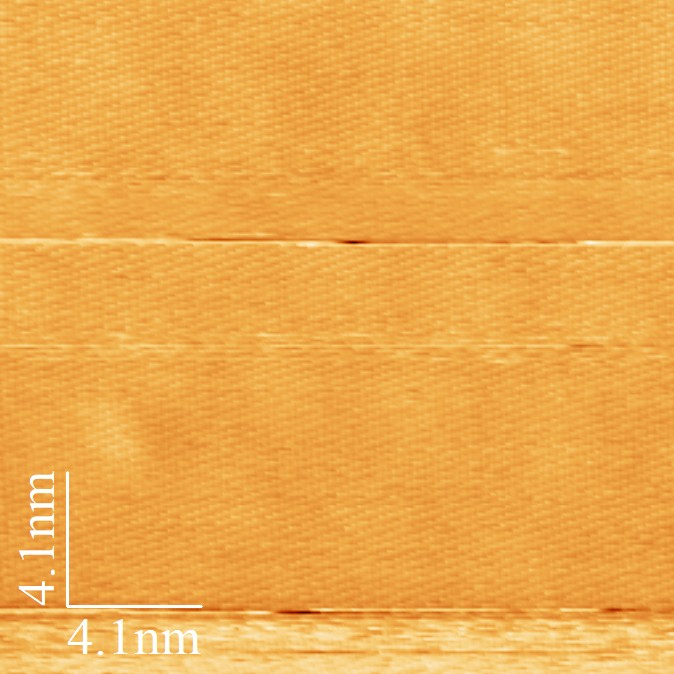
\includegraphics[width=0.45\linewidth]{2_muar_med}
	}
	\subfigure[]{
		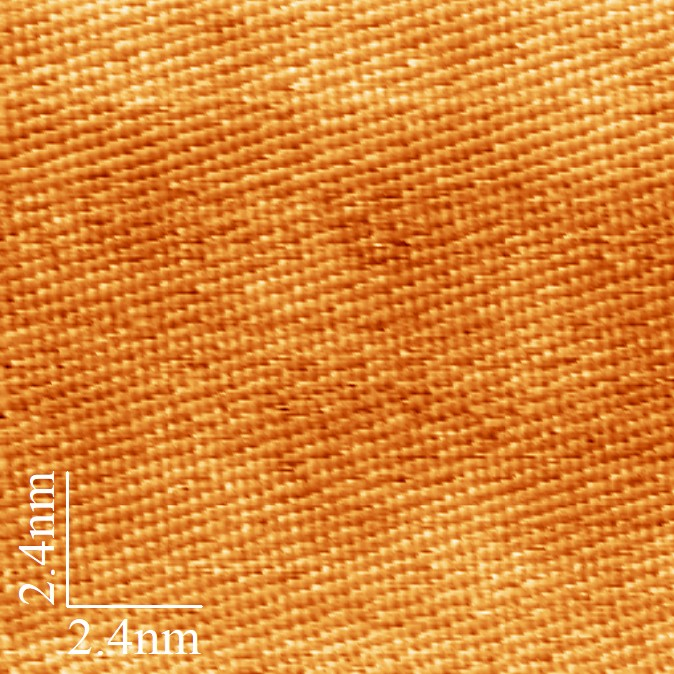
\includegraphics[width=0.7\linewidth]{2_muar_big}
	}
	\caption{СТМ-кадры графита с наблюдающимся муаром при различных увеличениях.}
	\label{fig:2_muar}
\end{figure}

\begin{figure}[H]
	\centering
	\subfigure[]{
		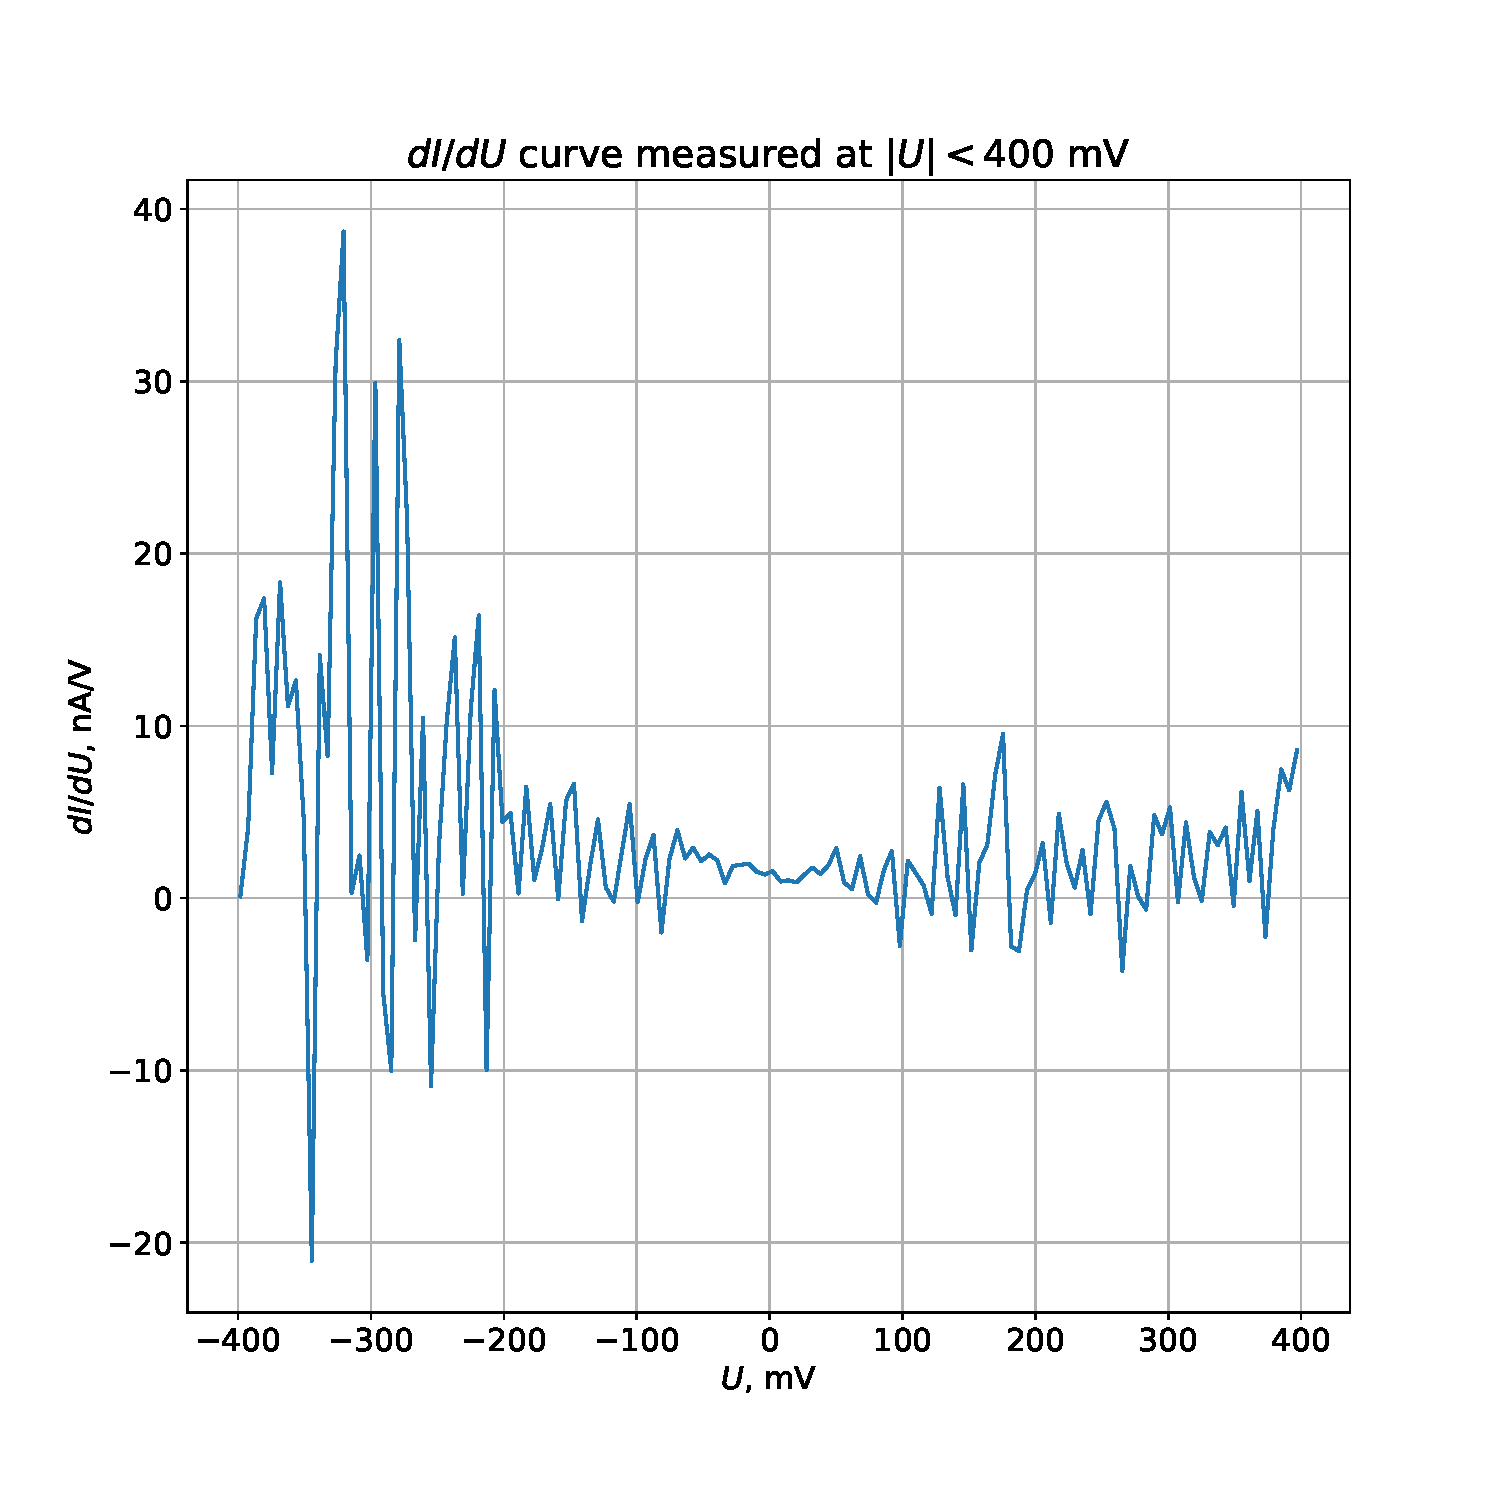
\includegraphics[width=0.6\linewidth]{3_curve}
	}
	\subfigure[]{
		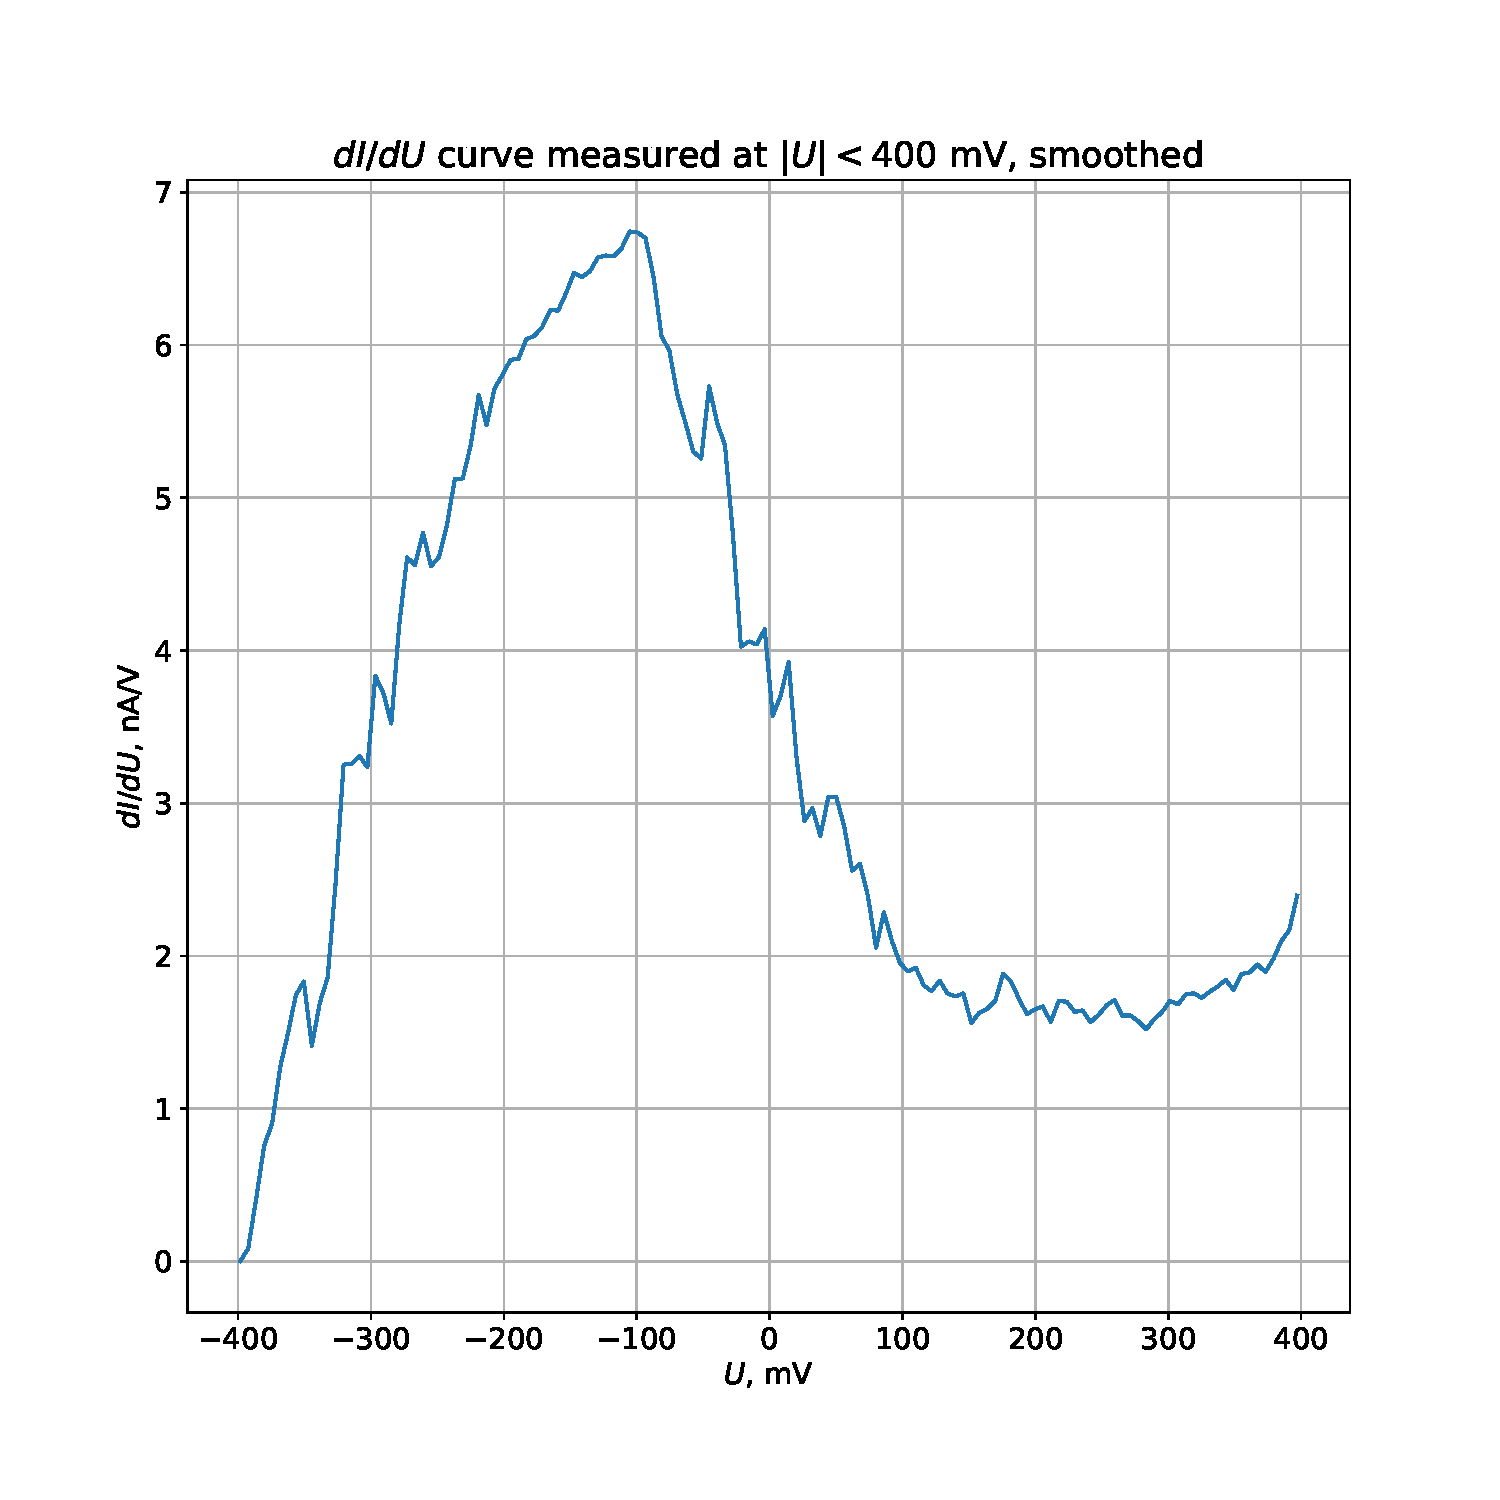
\includegraphics[width=0.6\linewidth]{3_curve_smooth}
	}
	\caption{Кривая $dI/dU$, измеренная при $|U| < 400$~mV (сверху) и она же, пропущенная через фильтр (снизу).}
	\label{fig:3_STS}
\end{figure}


































\end{document}